\section{Stochastic vehicle dynamics}
\label{sec:stochastic_vehicle_dynamics} 

We model the \emph{perturbed vehicle dynamics} as the following nonlinear continuous-time random dynamical system
\begin{align}
\dbx(t) = f(\bx(t), \bu(t)) + \bw(t),
\end{align}
where $\bu(t)$ are the deterministic control inputs, $\bw(t)$ is additive Gaussian white noise with zero mean and known covariance $\bQ(t)$, i.e. $\bw(t) \sim \calN(\bzero, \bQ(t))$, and the state $\bx(t)$ results in a Gaussian distribution with mean $\bmu(t)$ and covariance $\bP(t)$, so that $\bx(t) \sim \calN(\bmu(t), \bP(t))$.

Due to the symmetry of the probability density function (pdf) with respect to $\bmu(t)$, it is possible to represent the time evolution of the pdf as: i) the deterministic evolution of the mean $\bmu(t)$
\begin{align}
\dbmu(t) = f(\bmu(t), \bu(t)),
\end{align}
and ii) the time evolution of the state covariance matrix $\bP(t)$ along $\bmu(t)$, which can be expressed as
\begin{align}
\dbP(t) = \bA(t) \bP(t) + \bP(t) \bA^T(t) + \bQ(t),\quad \bP(0) = \bP_0.
\end{align}
The \emph{initial} state covariance $\bP_0$ is assumed known and $\bA(t)$ is the classical shorthand for the Jacobian along the mean trajectory $\bmu(t)$, that is $\bA(t)=\bJ(\bmu(t),\bu(t))$, where $\bJ(\bx, \bu) = \frac{\pd f(\bx, \bu)}{\pd \bx}$.

\begin{align}
\dbx = \begin{bmatrix}
              \dot{\bq}\\
              \dot{\bq}_v
             \end{bmatrix} =
             \begin{bmatrix}
              \bq_v\\
              \text{ABA}\text{dyn}(\bq, \bq_v, f_{xa}, f_{xb}, \delta, \bw),
             \end{bmatrix} = F(\bx).
	\label{eq:ABA_dyn}
\end{align}
               

The tangential forces exchanged between the tire and road are computed using \mbox{Pacejka's} \emph{Magic Formula}:
\begin{equation}\label{eqn_mf}
	[F_x,F_y]=\mf(\kappa,\alpha,F_z,\gamma),
\end{equation}
where $ F_x, F_y $ are the longitudinal and lateral forces, dependent on tire slips $( \kappa, \alpha )$, vertical load $( F_z )$, and camber angle $( \gamma )$.
As shown in Fig.~\ref{fig:tyre_wheel}, an auxiliary frame $\sref{N}$ is introduced to calculate $ F_z $. This depends upon the interpenetration $ d $ of the tire into the ground, following a penalty-based compliant tire model. This model treats the wheel as a radial spring-damper system with constant stiffness $ k_t $ and damping $ c_t $. The vertical force is expressed as:
\begin{equation}\label{eqn_Fz}
	F_z= F_0\log_2\left(1 + 2^{\frac{k_t d + c_t \dot{d}}{F_0}}\right)
\end{equation}
which is differentiable for $ d = 0 $ and $\dot{d} = 0$, improving numerical stability. The model ensures $ F_z $ approaches zero when the tire loses contact with the ground, while maintaining a non-zero gradient to guide optimization algorithms in scenarios where the tire detaches from the ground or encounters sudden changes.

%To compute the tangential components of the force exchanged by tyre and road, a formulation of the Pacejka's \emph{Magic Formula} ~\cite[Section~4.3.2]{Pacejka:book:2012} is used, which reads:
%\begin{equation}\label{eqn_mf}
%	[F_x,F_y]=\mf(\kappa,\alpha,F_z,\gamma).
%\end{equation}
%The Magic Formula $\mf$ computes the longitudinal and lateral forces $F_x,F_y$ as a function of the \emph{tyre slips} $\kappa,\alpha$~\cite[Section~1.2.1]{Pacejka:book:2012}. The formula is also sensitive to variations of vertical load $F_z$ and camber angle $\gamma$.
%
%The auxiliary frame $\sref{N}$ is introduced to compute quantities used in Eq.~\eqref{eqn_mf} and the (attempted) interpenetration $d$ (see Figure.~\ref{fig:tyre_wheel}) of the tyre in the ground, necessary to compute the dynamic vertical load $F_z$. The construction of the frame $\sref{N}$ is reported in Figure~\ref{fig:tyre_wheel}. It is worth noting that the frame $\sref{N}$ is fully described if $\sref{H}$ and $\sref{S}$ are known.
%The model used for the contact is a unilateral, penalty-based compliant tyre model, that considers the wheel as a radial spring with constant stiffness $k_t$ and constant damping coefficient $c_t$\footnote{The introduction of a more refined model with nonlinear spring and damping characteristics would not pose particular difficulties.}. The traditional role of compression in a spring is conducted by $d$, which is computed considering the road and the lowermost point of the non-deformed tyre. The resultant function that relate $d$, $\dot{d}$ and $F_z$ is:
%\begin{equation}\label{eqn_Fz}
%	F_z= F_0\log_2\left(1 + 2^{\frac{k_t d + c_t \dot{d}}{F_0}}\right)
%\end{equation}
%This function, with $F_0$ tuned to be negligible, is differentiable for $d=0$ and $\dot{d}=0$, enhancing numerical performance, and behaves as a spring-damper system, as requested, when the tyre is in contact with the ground. When the tyre detaches completely from the ground, the resultant vertical forces tends to zero. However, since its gradient is not zero, this formulation helps the optimization algorithm to figure out proper search directions. This allows to deal with jumps and other situations in which the tyre may lose contact with the ground.

\subsection{Camber System Modeling}
\label{sec:cambersystemmodeling}
The dynamic camber control (DCC) system is modeled as a simplified actuated revolute joint connecting the two virtual halves of the knuckle, though a real implementation might require a more complex 1-DoF joint. While this simplification may influence joint values from the optimizer, it results in nearly the same optimal wheel posture. The choice was driven by the limited literature on such systems for FSAE vehicles, which is the vehicle type employed in our analysis. A realistic model, if available, could be characterized using the same process applied to the suspension. During the design phase of the actual joint, some parameters could be treated as time-invariant optimization variables, constrained within dimensional bounds, to achieve the best performance configuration.
%The dynamic camber control (DCC) system is modeled here as a simple actuated revolute joint connecting the two virtual halves of the knuckle. A real implementation could require a more complex generalized 1-DoF joint. Changing the joint characteristics might affect the joint values obtained from the optimizer but would result in approximately the same optimal wheel posture. This simplification was necessary due to the limited open literature on such systems for FSAE vehicles. If a realistic model of the system were available, the process used for the suspension could easily be repeated to characterize this joint. It is worth observing that, in the design phase of the actual controlled joint, some model parameters could be treated as time-invariant optimization variables, appropriately constrained to meet dimensional bounds, and optimized to find the best performance configuration.

In Table~\ref{tab:camber_prop}, we report the range of variation of function $q_{hk}(t)$ and its first and second derivatives. Considering the scarcity of open literature available, reasonable values have been selected. In Figure~\ref{fig:camber_showing} the wheel is shown in a general posture with zero camber (shaded black) and with maximum positive camber (solid black). Due to the convention adopted for rotations, this posture corresponds to the minimum value of $q_{hk}$.
\begin{table}[h]
	\centering
	\begin{tabular}{|c|c|c|}
		\hline
		$q_{hk}$ (rad) & $\dot{q}_{hk}$ (rad/s)& $\ddot{q}_{hk}$ (rad/s$^2$)\\\hline
		$\pm \pi/20$ & $\pm \pi/20$ & $\pm \pi/10$ \\\hline
	\end{tabular}
	\caption{Upper and lower bounds for camber angle value $q_{hk}(t)$ and its derivatives.}
	\label{tab:camber_prop}
\end{table}

\begin{figure}[h]
	\centering
	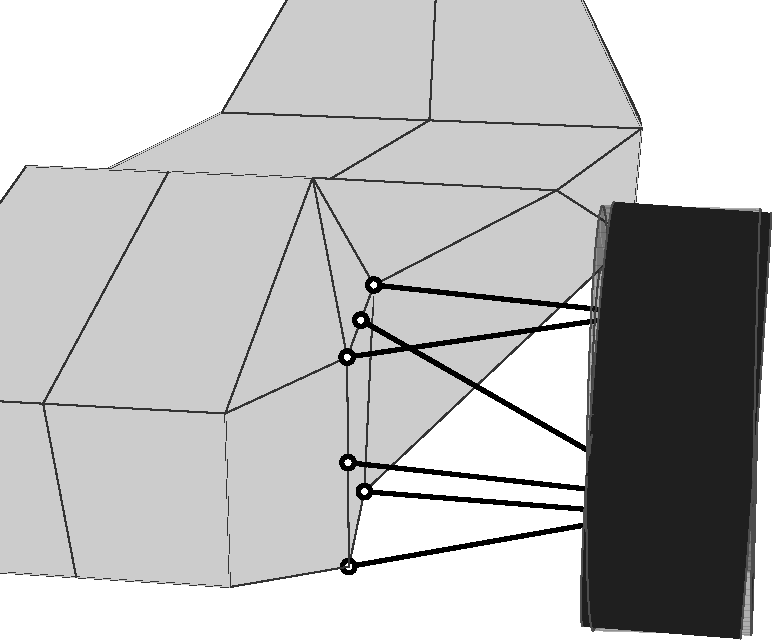
\includegraphics[scale = .6]{Images/camber_showing}
	\caption{Real scale representation of the wheel in two configurations: $q_{hk}=0$ (shaded surface) and $q_{hk}=-\pi/20$ (solid surface).}
	\label{fig:camber_showing}
\end{figure}
\subsection{External Wrenches}
\label{sec:extwren}
The external wrenches acting on each body, from wheels to chassis, are expressed in body-fixed components. Only gravity, aerodynamic forces, and road-tyre interactions are considered. Following~\cite{Guiggiani:book:2023}, the aerodynamic wrench in frame $\{B\}$ is $W_a=-\frac{1}{2}\rho S v_{gb,1}^2 [C_x, 0, C_z, 0, -h_0 C_x - a_f C_{zf} + a_r C_{zr}, 0]^T$, where $\rho$ is air density, $S$ is the frontal area, $v_{gb,1}$ the forward velocity (component of \emph{distal rigid-body twist} $V_{gb}$, see~\cite[p.~4]{Domenighini:Designs:2023}), and $C_x, C_z$ are drag/lift coefficients. $C_z$ is split into $C_{zf}=k_a C_z$ and $C_{zr}=(1-k_a)C_z$ by the aerodynamic balance coefficient $k_a$.

The total external wrench on a wheel is $W_{we}=\Ad_{g_{hn}}^*W_t+W_{w_h}$,
%\begin{equation}\label{eqn:Wwe}
%W_{we}=\Ad_{g_{hn}}^*W_t+W_{w_h},
%\end{equation}
where $W_t=[F_x, F_y, F_z, 0, 0, 0]^T$ is the ground wrench transferred from $\sref{N}$ to $\sref{H}$ by the \emph{starred} Adjoint operator, and $W_{w_h}=[F_{w_h}^T R_{hg}^T, 0, 0, 0]^T$ is the weight contribution with $F_{w_h}=[0, 0, -m_h g]^T$ in frame $\{G\}$, where $m_h$ is the wheel mass.

Knuckles experience no external forces, therefore:
\begin{equation}\label{eqn:Whe}
	W_{he}=[0,0,0,0,0,0]^T\quad\textrm{and}\quad W_{ke}=[0,0,0,0,0,0]^T.
\end{equation}
The chassis's external wrench is $W_{be}=W_a+W_{w_b}$, %\begin{equation}\label{eqn:Wbe}
%	W_{be}=W_a+W_{w_b},
%\end{equation}
where $W_a$ and $W_{w_b}$ are aerodynamic and weight contributions, respectively. For $W_{w_b}=[F_{w_b}^T R_{bg}^T, 0, 0, 0]^T$, the weight force is $F_{w_b}=[0, 0, -m_b g]^T$ in frame $\{G\}$, with $m_b$ as the chassis mass.
%The purpose of this section is to describe the external wrenches acting on each body, from the wheels to the chassis, each expressed in body-fixed components.
%Besides gravity, aerodynamic forces and the interactions between road and tyres are the only external forces considered.
%Adopting the notation in~\cite{Guiggiani:book:2023}, the aerodynamic contribution to the wrenches in frame $\{B\}$ is $W_a=-\frac{1}{2}\rho Sv_{gb,1}^2[C_x,0,C_z,0,-h_0C_x-a_fC_{zf}+a_rC_{zr},0]^T$, where $\rho$ is the air density, $S$ the frontal area of the vehicle, $v_{gb,1}$ the forward velocity, $h_0$ the nominal height of the CoM from ground and $a_f,a_r$ the distances of the CoM from the front and rear axle, respectively. The drag and lift coefficient $C_x$ and $C_z$ are dimensionless parameters that depend on the shape of the vehicle's body. $C_z$ can be further partitioned into $C_{zf}=k_a C_z$ and $C_{zr}=(1-k_a) C_z$ according to the \emph{aerodynamic balance coefficient} $k_a$, which is a parameter of the vehicle set-up.
%
%The total external wrench acting on a (general) wheel is:
%\begin{equation}\label{eqn:Wwe}
%	W_{we}=\Ad_{g_{hn}}^*W_t+W_{w_h},
%\end{equation}
%where $W_t=[F_x,F_y,F_z,0,0,0]^T$ are the ground forces computed in $\sref{N}$ and properly transferred to $\sref{H}$ components by the \emph{starred} Adjoint operator, while $W_{w_h} = [ F_{w_h}^T R^T_{hg}, 0,0,0 ]^T$, with $F_{w_h}=[0,0,-m_h g]^T$ in frame $\{G\}$, represents the weight contribution and $m_{h}$ is the wheel mass.
%
%Under our hypotheses, the knuckles are not subjected to external forces, thus \begin{equation}\label{eqn:Whe}
%	W_{he}=[0,0,0,0,0,0]^T\quad\textrm{and}\quad W_{ke}=[0,0,0,0,0,0]^T.
%\end{equation}
%
%The resultant external wrench acting on the chassis is therefore:
%\begin{equation}\label{eqn:Wbe}
%	W_{be}=W_a+W_{w_b},
%\end{equation}
%where $W_a$ and $W_{w_b}$ are, respectively, the contributions of aerodynamic and chassis weight forces, whose general expression is of the form $W_{w_b} = [ F_{w_b}^T R^T_{bg}, 0,0,0 ]^T$. Explicitly we have $F_{w_b}=[0,0,-m_b g]^T$ in frame $\{G\}$, where $m_b$ is the mass of the chassis.

\subsection{Recursive computation of the dynamics equations with ABA}
\label{sec:aba}
Thanks to the ABA algorithm, assuming known joint positions and velocities and joint forces and torques, it is possible to compute recursively and efficiently the accelerations of the joint variables. Following~\cite{Domenighini:Designs:2023}, twists are streamlined as follows: $V_{gb}^b = V_{gb} = V_b$, $V_{bh}^h=V_{bh}$, $V_{hw}^h=V_{hw}$. For the second model (DCC) the last expression is replaced with $V_{kw}^k=V_{kw}$ and $V_{hk}^k=V_{hk}$ is added. Given that the first model (without camber control) is a particular case of the DCC one, to avoid duplications only the algorithm for DCC is reported here.

The traditional ABA requires knowledge of the active forces and torques, denoted as $\tau_{ij}$, exerted by the parent body ($i$) on the child body ($j$). Its purpose is to solve the \emph{Forward Dynamics} problem of an articulated systems of rigid bodies. In our floating-base system, given the twist $V_b$ of the parent body $\{B\}$, the values and time derivatives of all joint variables ($q$ and $\dot{q}$), and the torque vector ($\tau$), the objective is to compute the joint accelerations ($\dot{V}_{b}$ and $\ddot{q}$).
%The fundamental concept is that of the inertia of an articulated body. This is represented by that of the root rigid body (original parent) plus the portion of the sub-trees, composed by the children bodies, whose inertia that can be structurally transferred backwards through the joints.
%This depends on the architecture, the pose and the joints' types.
The overall computation is performed in three sweeps defined recursively. One of the greatest computational benefits when it is employed to assemble symbolic dynamic equations, as in our case, is that \emph{no matrix inversion is required}, thus contributing to streamline the algebraic expressions.

The first step of the algorithm, as described in \textbf{Step 1}, performs the forward propagation of rigid-body velocities: from the root to the leaves of the tree.
%Twists are calculated as the sum of parent twist and the relative twist which is expressed consistently with the joint type. The interesting Jacobians are listed here: $J_{hk}=[0,0,0,1,0,0]^T$ and $J_{kw}=[0,0,0,0,1,0]^T$, and represent two revolute joints with axes $x$ and $y$ respectively.
In Algorithm~\ref{alg:step1} the terms ``Knuckle 1'' and ``Knuckle 2'' are used to identify the two halves of the knuckle, where, using kinematic trees terminology, the first is the parent of the second.
The Adjoint operator is defined as follows:
\begin{equation}\label{eq:Adjoint} \Ad_{g}=\left[\begin{array}{cc}R&\hat{d}R\\0&R\end{array}\right].
\end{equation}
In the case $g_{bh}\in SE(3)$ is considered, $R_{bh}\in SO(3)$ and $d_{bh}\in \bbR^3$ are functions of $(z,\delta)$. In the case of $g_{hk}$, the expressions are simply $d_{hk}=[0,0,0]^T$ and $R = \rotX(q_{hk})$, the latter being an elementary rotation about the common $x$-axis of the angle $q_{hk}$.

\begin{algorithm}[h]
	\floatname{algorithm}{Step}
	\caption{Forward Propagation of Velocity}\label{alg:step1}
	\begin{algorithmic}[1]
		\vspace{1mm}
		\For{$h=h_1,h_2,h_3,h_4$}
		\vspace{1mm}
		\State{$V_{bh}=J_{bh,z}\dot{z}+J_{bh,\delta}\dot{\delta}$}
		\vspace{1mm}
		\State{$V_h=\Ad_{g_{bh}}^{-1}V_b+V_{bh}$}\Comment{Knuckle 1 Rigid-Body Velocity}
		\vspace{1mm}
		\State{$V_{hk} = J_{hk}\dot{q}_{hk}$}
		\vspace{1mm}
		\State{$V_k=\Ad_{g_{hk}}^{-1}V_h+V_{hk}$}\Comment{Knuckle 2 Rigid-Body Velocity}
		\vspace{1mm}
		\State{$V_{kw}=J_{kw}\omega$}
		\vspace{1mm}
		\State{$V_w=V_k+V_{kw}$}\Comment{Rim Rigid-Body Velocity}
		\vspace{1mm}
		\EndFor
		\vspace{1mm}
	\end{algorithmic}
\end{algorithm}

The second step of the algorithm, as detailed in \textbf{Step 2}, performs the backward propagation of inertia and bias terms.
\begin{algorithm}[h]
	\floatname{algorithm}{Step}
	\caption{Backward Propagation of Articulated Inertia and Bias}\label{alg:step2}
	\begin{algorithmic}[1]
		\vspace{1mm}
		\For{$h=h_1,h_2,h_3,h_4$}
		\vspace{1mm}
		\State{$\hat{M}_w=M_w$}\Comment{Rim Articulated Inertia}
		\vspace{1mm}
		\State{$\hat{B}_w=-W_{we}+\ad_{V_w}^*M_wV_w$}\Comment{Rim Articulated Bias}
		\vspace{1mm}
		\State{$\bar{M}_w=\hat{M}_w-\dfrac{\hat{M}_wJ_{hw}J_{hw}^T\hat{M}_w}{J_{hw}^T\hat{M}_wJ_{hw}}$}
		\vspace{1mm}
		\State{$\bar{B}_w=\hat{B}_w-\dfrac{\hat{M}_wJ_{hw}J_{hw}^T\hat{B}_w}{J_{hw}^T\hat{M}_wJ_{hw}}-\bar{M}_w\ad_{V_{hw}}V_w$}
		\vspace{1mm}
		\State{$\hat{M}_k= \bar{M}_w$
		}\Comment{Knuckle 2 Articulated Inertia}
		\vspace{1mm}
		\State{$\hat{B}_k= \bar{B}_w$
		}\Comment{Knuckle 2 Articulated Bias}
		\vspace{1mm}
		\State{$\hat{M}_h= \Ad_{g_{hk}}^*\hat{M}_k\Ad_{g_{hk}}^{-1}$
		}\Comment{Knuckle 1 Articulated Inertia}
		\vspace{1mm}
		\State{$\hat{B}_h= \Ad_{g_{hk}}^*\bigl(\hat{M}_k(J_{hk}\ddot{q}_{hk}-\ad_{V_{hk}}\Ad_{g_{kh}}V_k)+\hat{B}_k\bigr)$
		}\Comment{Knuckle 1 Articulated Bias}
		\vspace{1mm}
		\State{$\bar{M}_h=\hat{M}_h-\dfrac{\hat{M}_hJ_{bh,z}J_{bh,z}^T\hat{M}_h}{J_{bh,z}^T\hat{M}_hJ_{bh,z}}$}
		\vspace{1mm}
		\State{$\bar{B}_h=\hat{B}_h-\dfrac{\hat{M}_hJ_{bh,z}(J_{bh,z}^T\hat{B}_h-\tau)}{J_{bh,z}^T\hat{M}_hJ_{bh,z}}-\bar{M}_h(\ad_{V_{bh}}V_h-\dot{J}_{bh,z}\dot{z}-\dot{J}_{bh,\delta}\dot{\delta}-J_{bh,\delta}\ddot{\delta})$}
		\vspace{1mm}
		\EndFor
		\vspace{1mm}
		\State{$\hat{M}_b=M_b+\displaystyle\sum_h\Ad_{g_{bh}}^*\bar{M}_h\Ad_{g_{bh}}^{-1}$}\Comment{Chassis Articulated Inertia}
		\vspace{1mm}
		\State{$\hat{B}_b=-W_{be}+\ad_{V_b}^*M_bV_b+\displaystyle\sum_h\Ad_{g_{bh}}^*\bar{B}_h$}\Comment{Chassis Articulated Bias}
		\vspace{1mm}
	\end{algorithmic}
\end{algorithm}

%Both inertia and bias are expressed in the body-fixed components.
In the case the DCC architecture is considered, the camber angle acceleration $\ddot{q}_{hk}$ is known, since $q_{hk(t)}$ is the assumed input, while the torque $\tau_{hk}$ has to be computed together with the rest of unknown accelerations, which are the outcome of the third sweep. This leads to a \emph{Hybrid Dynamics} problem that requires to carefully revisit the ABA's second and third steps.
The approach used is inspired by~\cite[Section~2.3]{Kim:notes:2012} where the the notation and conventions here employed were adapted according to~\cite{Domenighini:Designs:2023}.
%Specifically, apart from the labels assigned to the quantities, the primary difference between the two methods is the ordering of the twist vector. In this work, the twist vector is defined as $V = [v,\omega]^T$, whereas in the other method, it is defined as $V=[\omega,v]^T$. This difference might seem minor but leads to significant changes in the definitions of Adjoint operators, inertia matrices, bias and wrench vectors.

%For a generic articulated body the Newton-Euler equations can be expressed in the form:
%\begin{equation}\label{eqn:NE}
%	W=\hat{M}\dot{V}+\hat{B}.
%\end{equation}
%For a leaf node of the kinematic tree, having no children, the articulated inertia $\hat{M}$ is simply the generalized inertia $M$ of the body itself. Consistently, the bias $\hat{B}=B$, where:
%\begin{equation}
%	B=-W_e+\ad_V^*MV,
%\end{equation}
%and where $W_e$ is the resultant external wrench applied to the body and $\ad_V^*MV$ accounts for generalized gyroscopic and centrifugal forces, which are bi-linear in $V$. According to~\cite[Section~4.3.3]{Murray:book:1994} $\ad^*=-\ad^T$ has been defined. (If $v$ and $\omega$ are the translational and rotational component of $V$, then $\ad^*_V=\left[\begin{smallmatrix}\hat{\omega}&0\\\hat{v}&\hat{\omega}\end{smallmatrix}\right]$).

Starting from the leaf nodes, which in our case are represented by the wheels ($\sref{W}$), after providing information such as external wrenches, twists, joint geometry, body masses, joint forces / torques for traditional connections, and time evolution of variables defining kinematically imposed joints, the backward propagation of inertia and bias can be performed.

Finally the last step, denoted as \textbf{Step 3}, starting from the root node, computes joint variable accelerations and consequently body twists derivatives. For the kinematically controlled camber joints, the torques $\tau_{hk}$ needed to maintain the desired state of motion (DCC architecture) are computed as a by-product of the local inverse dynamics. This information is crucial to prevent actuators from  saturating or operating outside their bandwidth in the planned trajectories.

The root twist acceleration is determined by solving equation $W=\hat{M}\dot{V}+\hat{B}$, considering that the chassis is free-floating. The other unknown quantities, such as variable accelerations and torques, are computed projecting the Newton-Euler equations of each body along the respective Jacobian and then solving for the variable. See also~\cite{Domenighini:Designs:2023} for more details in the derivation of the equations.

\begin{algorithm}[h]
	\floatname{algorithm}{Step}
	\caption{Forward Propagation of Acceleration}\label{alg:step3}
	\begin{algorithmic}[1]
		\State{$\dot{V}_b=-\hat{M}_b^{-1}\hat{B}_b$}\Comment{Chassis Rigid-Body Acceleration}
		\vspace{1mm}
		\For{$h=h_1,h_2,h_3,h_4$}
		\vspace{1mm}
		\State{$\ddot{z}=-\dfrac{J_{bh,z}^T\bigl(\hat{B}_h+\hat{M}_h(\Ad_{g_{bh}}^{-1}\dot{V}_b-\ad_{V_{bh}}V_h+\dot{J}_{bh,z}\dot{z}+\dot{J}_{bh,\delta}\dot{\delta}+J_{bh,\delta}\ddot{\delta})\bigr)-\tau}{J_{bh,z}^T\hat{M}_hJ_{bh,z}}$}
		\vspace{1mm}
		\State{$\dot{V}_{bh}=\dot{J}_{bh,z}\dot{z}+\dot{J}_{bh,\delta}\dot{\delta}+J_{bh,z}\ddot{z}+J_{bh,\delta}\ddot{\delta}$}
		\vspace{1mm}
		\State{$\dot{V}_h=\Ad_{g_{bh}}^{-1}\dot{V}_b-\ad_{V_{bh}}V_h+\dot{V}_{bh}$}\Comment{Knuckle 1 Rigid-Body Acceleration}
		\vspace{1mm}
		\State{$\tau_{hk} = J_{hk}^T\bigl(\hat{B}_k+\hat{M}_k(\Ad_{g_{kh}}\dot{V}_h-\ad_{V_{hk}}V_k + J_{hk}\ddot{q}_{hk})\bigr)$}
		\vspace{1mm}
		\State{$\dot{V}_{bh} = J_{hk}\ddot{q}_{hk}$}
		\vspace{1mm}
		\State{$\dot{V}_k=\Ad_{g_{hk}}^{-1}\dot{V}_h-\ad_{V_{hk}}V_k+\dot{V}_{bh}$}\Comment{Knuckle 2 Rigid-Body Acceleration}
		\State{$\dot{\omega}=-\dfrac{J_{kw}^T\bigl(\hat{B}_w+\hat{M}_w(\dot{V}_k-\ad_{V_{kw}}V_w)\bigr)}{J_{kw}^T\hat{M}_wJ_{kw}}$}
		\vspace{1mm}
		\EndFor
		\vspace{1mm}
	\end{algorithmic}
\end{algorithm}

\subsection{Dynamic Model}
The dynamics equations, assembled via the procedure described  in Sec.~\ref{sec:aba}, are implemented in the software code by using a state-space representation $\dot{x}=f(x,u)$.
%\begin{equation}\label{eqn:f}
%	\dot{x}=f(x,u).
%\end{equation}
The state vector is $x = (q_{gb};V_{gb};z;\dot{z};\omega;q_{hk};\dot{q}_{hk})\in\bbR^{32}$, with components defined in previous sections. As already mentioned, in the model the camber joint is kinematically controlled as per the DCC architecture. Hence, the associated control vector is $u=(T_a;T_b;\delta;\ddot{q}_{hk})\in\bbR^{16}$, where each element is in $\bbR^{4}$ and collects the controls of the branch to each wheel. The torque is split into acceleration and braking components, allowing for minor modifications to model on-board motors coupled with traditional brakes and/or in-wheel motors as well. These components have their reaction torques in two different bodies in case of on-board motors and traditional brakes: the chassis and the knuckles, respectively. The $\delta$ vector collects the four translations of the steering rod attachment points, as described in Section~\ref{sec:suspanal}, while for the vector $\ddot{q}_{hk}$ no further explanation should be necessary. Clearly, this representation is valid for the model with active camber. The simpler model (no DCC) shares with the former the first 24 components of the state vector and the first 12 of the control vector.

The time derivative of the state vector has also been expressed previously except for the first element, $q_{gb}$. Its derivative is a function of the state and can be recovered using a standard procedure~\cite{Domenighini:Designs:2023} as follows:
\begin{equation}\label{eqn:dotqgb}
	\dot{q}_{gb}=J_{gb}^{-1}(q_{gb})V_{gb},
\end{equation}
where $J_{gb}(q_{gb})\in\bbR^{6\times6}$ is the Jacobian of the virtual joint connecting the ground to the chassis, and it is computed via the PoE parameterization of the transformation $g_{gb}$.
%, similarly to $J_{bh}$ in Eq.~\eqref{eqn:Jbh}. 